\documentclass[a5paper]{memoir}
\usepackage[hidelinks]{hyperref}
\usepackage{memhfixc}
%\makeatletter
%\newcommand*{\currentname}{\@currentlabelname}
%\makeatother

\usepackage[calc]{adjustbox}
\usepackage{lipsum}
\usepackage{wrapfig}
\usepackage{cutwin}
\usepackage{amsthm}
\usepackage{amsmath}
\usepackage{amssymb}
\usepackage{tikz}
\usepackage[shortlabels]{enumitem}
\usetikzlibrary{calc,intersections,through,backgrounds}
%\renewcommand*\rmdefault{dayroms}
\usepackage[T1]{fontenc}
\usepackage{titlesec}
%\usepackage{lua-visual-debug}
\setcounter{tocdepth}{3}
\usepackage{lettrine}
\usepackage{wrapfig}
%%%%%%%%
\makepagestyle{euclidbasic}
\makeevenhead{euclidbasic}{\thepage}{BOOK \thechapter. \nameref{section\thesection}.}{}
\makeoddhead{euclidbasic}{}{BOOK \thechapter. \nameref{section\thesection}.}{\thepage}

\makepagestyle{euclidprob}
\makeevenhead{euclidprob}{\thepage}{BOOK \thechapter. PROP. \theprop. PROB.}{}
\makeoddhead{euclidprob}{\thepage}{BOOK \thechapter. PROP. \theprop. PROB.}{}

\makepagestyle{euclidthm}
\makeevenhead{euclidthm}{\thepage}{BOOK \thechapter. PROP. \theprop. THEOR.}{}
\makeoddhead{euclidthm}{\thepage}{BOOK \thechapter. PROP. \theprop. THEOR.}{}

\makepagestyle{euclidintro}
\makeevenhead{euclidintro}{}{INTRODUCTION.}{\thepage}
\makeoddhead{euclidintro}{\thepage}{INTRODUCTION.}{}

%%%%%%%%

\titleformat{\chapter}
{\centering\normalfont}{Book~\thechapter}{1em}{}
\titleformat{\section}
{\centering\normalfont}{}{1em}{}
\titleformat{\subsection}
{\centering\normalfont}{}{1em}{}
\renewcommand{\subsection}[1]{%
  \par\refstepcounter{subsection}% Increase section counter
  \sectionmark{#1}% Add section mark (header)
  \addcontentsline{toc}{subsection}{\protect\numberline{\thesubsection}#1}% Add section to ToC
}
%\theoremstyle{plain}
%\newtheorem{prop}{}
\newenvironment{prop}[1]{#1\begin{itshape}\refstepcounter{prop}\label{prop\theprop}}{\end{itshape}}
\newcounter{prop}
\renewcommand{\qedsymbol}{Q.E.D.}
\newenvironment{bizarrelist}
 {\enumerate[
    align=left,
    leftmargin=0pt,
    labelwidth=0pt,
    label={\makebox[\textwidth][c]{\Roman*.}},
    ref=\arabic*,
    before=\changeitem,
 ]}
 {\endenumerate}
\newcommand{\changeitem}{\let\saveditem\item\def\item{\saveditem\mbox{}\\*}}

\definecolor{blue}{rgb}{0.13, 0.67, 0.8}
\definecolor{yellow}{rgb}{1.0, 0.75, 0.0}
\definecolor{red}{rgb}{0.92, 0.3, 0.26}
\usepackage{corners}
\newcommand{\tikzhline}[2][black]{ 
\tikz[baseline=-0.5ex]\draw[ultra thick,#1] (0,0) -- (#2,0);
}
\newcommand{\tikzsector}[4][black]{ 
\tikz[minimum height=2em,scale=0.4]\fill[#1] (0,0) -- (#2:#4) arc (#2:#3:#4) -- cycle;
}
\DeclareDocumentCommand{\tikztriangle}{O{black} O{black} O{black} m m m}{
    \tikzcorner[#1][#2]{#4}{#5}{#6}
    \tikzcorner[#2][#3]{#5}{#6}{#4}
    \tikzcorner[#3][#1]{#6}{#4}{#5}
}
\newcommand{\refprop}[1]{pr. \ref{prop#1}.}
\newcommand{\refdef}[1]{def. \ref{def#1}.}
\newcommand{\refax}[1]{ax. \ref{ax#1}.}
\newcommand{\refpost}[1]{post. \ref{post#1}.}
\newcommand{\manydots}[2][9pt]{
\begin{tikzpicture}
\foreach \x in {1,...,#2} 
\fill (\x*#1,0) circle (0.55pt);
\end{tikzpicture}
}

\renewcommand{\therefore}{
\ensuremath{
\mathrel{
\begin{tikzpicture}[scale=0.18]
\fill (0,0) circle (5pt);
\fill (1,0) circle (5pt);
\fill (60:1) circle (5pt);
\end{tikzpicture}} }}

\renewcommand{\because}{
\ensuremath{
\mathrel{
\begin{tikzpicture}[scale=-0.18]
\fill (0,0) circle (5pt);
\fill (1,0) circle (5pt);
\fill (60:1) circle (5pt);
\end{tikzpicture}} }}

\newcommand{\equals}{
\ensuremath{
\mathrel{
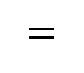
\begin{tikzpicture}[baseline=-1.0ex]
\draw[line width=1.0pt] (0,1.5pt) -- (9pt,1.5pt);
\draw[line width=1.0pt] (0,-1.5pt) -- (9pt,-1.5pt);
\end{tikzpicture}}}
}

\newcommand{\notequals}{
\ensuremath{
\mathrel{

\begin{tikzpicture}[baseline=-0.5ex]
\draw[line width=1.0pt] (0,1.5pt) -- (9pt,1.5pt);
\draw[line width=1.0pt] (0,-1.5pt) -- (9pt,-1.5pt);
\draw[line width=1.0pt] (4.5pt,-4pt) -- (4.5pt,4pt);
\end{tikzpicture}}}
}

\newcommand{\greater}{
\ensuremath{
\mathrel{

\begin{tikzpicture}
\draw[line width=1.0pt] (9pt,2.5pt) -- (0,2.5pt) -- (0,-2.5pt) -- (9pt,-2.5pt);
\end{tikzpicture}}}
}
\newcommand{\less}{
\ensuremath{
\mathrel{

\begin{tikzpicture}[scale=-1]
\draw[line width=1.0pt] (9pt,2.5pt) -- (0,2.5pt) -- (0,-2.5pt) -- (9pt,-2.5pt);
\end{tikzpicture}}}
}
\newcommand{\notgreater}{
\ensuremath{
\mathrel{

\begin{tikzpicture}
\draw[line width=1.0pt] (9pt,2.5pt) -- (0,2.5pt) -- (0,-2.5pt) -- (9pt,-2.5pt);
\draw[line width=1.0pt] (4.5pt,-5pt) -- (4.5pt,5pt);
\end{tikzpicture}}}
}
\newcommand{\notless}{
\ensuremath{
\mathrel{

\begin{tikzpicture}[scale=-1]
\draw[line width=1.0pt] (9pt,2.5pt) -- (0,2.5pt) -- (0,-2.5pt) -- (9pt,-2.5pt);
\draw[line width=1.0pt] (4.5pt,-5pt) -- (4.5pt,5pt);
\end{tikzpicture}}}
}
\newcommand{\plus}{
\ensuremath{
\mathbin{
\begin{tikzpicture}
\draw[line width=1.0pt] (0pt,-4pt) -- (0pt,4pt);
\draw[line width=1.0pt] (-4pt,0pt) -- (4pt,0pt);
\end{tikzpicture}}}
}
\newcommand{\minus}{
\ensuremath{
\mathbin{
\begin{tikzpicture}
\draw[line width=1.0pt] (-4pt,0pt) -- (4pt,0pt);
\end{tikzpicture}}}
}
\newcommand{\cross}{
\ensuremath{
\mathbin{

\begin{tikzpicture}[rotate=45]
\draw[line width=1.0pt] (0pt,-4pt) -- (0pt,4pt);
\draw[line width=1.0pt] (-4pt,0pt) -- (4pt,0pt);
\end{tikzpicture}}}
}
\newcommand{\isto}{
\ensuremath{
\mathrel{
\begin{tikzpicture}
\fill (0,1.5pt) circle (1pt);
\fill (0,-1.5pt) circle (1pt);
\end{tikzpicture}}}
}
\newcommand{\as}{
\ensuremath{
\mathrel{

\begin{tikzpicture}
\fill (-1.5pt,1.5pt) circle (1pt);
\fill (-1.5pt,-1.5pt) circle (1pt);
\fill (1.5pt,1.5pt) circle (1pt);
\fill (1.5pt,-1.5pt) circle (1pt);
\end{tikzpicture}}}
}

\newcommand{\plel}{
\ensuremath{
\mathrel{

\begin{tikzpicture}
\draw[line width=1pt] (-1.2pt,-4.0pt) -- (-1.2pt,4.0pt);
\draw[line width=1pt] (1.2pt,-4.0pt) -- (1.2pt,4.0pt);
\end{tikzpicture}}}
}
\newcommand{\perpendicular}{
\ensuremath{
\mathrel{
\begin{tikzpicture}
\draw[line width=1pt] (0pt,6.0pt) -- (0pt,0pt);
\draw[line width=1pt] (-4.0pt,0pt) -- (4.0pt,0pt);
\end{tikzpicture}}}
}

\newcommand{\acuteangle}{

\begin{tikzpicture}[thick]
\draw (0,0) -- (18pt,0) arc (0:40:18pt) -- cycle;
\end{tikzpicture}
}
\newcommand{\rightangle}{

\begin{tikzpicture}[thick]
\draw (0,0) -- (18pt,0) arc (0:90:18pt) -- cycle;
\end{tikzpicture}
}
\newcommand{\rightangles}{
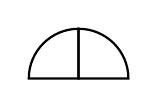
\begin{tikzpicture}[thick]
\draw (0,0) -- (18pt,0) arc (0:90:18pt) -- cycle;
\draw (0,0) -- (0,18pt) arc (90:180:18pt) -- cycle;
\end{tikzpicture}
}
\newcommand{\vertex}{

\begin{tikzpicture}[scale=0.35,ultra thick,rotate=-93]
\draw (0,0) -- (1,0) -- (0,0) -- (40:1);
\end{tikzpicture}
}
\newcommand{\trivertex}{

\begin{tikzpicture}[scale=0.6,ultra thick,rotate=-130]
\clip[rotate=130] (-1,-0.6) rectangle (0.7,0.1);
\draw (90:1) -- (0,0) -- (1,0);
\draw (1,0) -- (0,0) -- (90:1);
\draw (0,0) -- (40:1);
\end{tikzpicture}
}


\begin{document}
    %\pagestyle{empty}
    \pagestyle{euclidintro}
    \frontmatter
    \tableofcontents
        \chapter{INTRODUCTION.}
    \lettrine[lines=2]{T}{HE arts and sciences have} become so extensive,
    that to facilitate their acquirement is of as much importance as to
    extend their boundaries. Illustration, if it does not shorten the time
    of study, will at least make it more agreeable. \textsc{This work} has
    a greater aim than mere illustration; we do not introduce colours for
    the purpose of entertainment, or to amuse \textit{by certain
    combinations of tint and form}, but to assist the mind in its
    researches after truth, to increase the facilities of instruction, and
    to diffuse permanent knowledge. If we wanted authorities to prove the
    importance and usefulness of geometry, we might quote every
    philosopher since the days of Plato. Among the Greeks, in ancient, as
    in the school of Pestalozzi and others in recent times, geometry was
    adopted as the best gymnastic of the mind. In fact, Euclid's Elements
    have become, by common consent, the basis of mathematical science all
    over the civilized globe. But this will not appear extraordinary, if
    we consider that this sublime science is not only better calculated
    than any other to call forth the spirit of inquity, to elevate the
    mind, and to strengthen the reasoning faculties, but also it forms the
    best introduction to most of the useful and important vocations of
    human life. Arithmetic, land-surveying, mensuration, engineering,
    navigation, mechanics, hydrostatics, pneumatics, optics, physical
    astronomy, \&c. are all dependent on the propositions of geometry. 

    Much however depends on the first communication of any science to a
    learner, though the best and most easy methods are seldom adopted.
    Propositions are placed before a student, who though having a
    sufficient understanding, is told just as much about them on entering
    at the very threshold of the science, as gives gives him a
    prepossession most unfavourable to his future study of this delightful
    subject; or the formalitites and paraphernalia of rigour are so
    ostentatiously put forward, as almost to hide the reality. Endless and
    perplexing repetitions, which do not confer greater exactitude on the
    reasoning, render the demonstrations involved and obscure, and conceal
    from the view of the student the consecution of evidence.'' Thus an
    aversion is created in the mind of the pupil, and a subject so
    calculated to improve the reasoning powers, and give the habit of
    close thinking, is degraded by a dry and rigid memory, To raise the
    curiosity, and to awaken the listless and dormant powers of younger
    minds should be the aim of every teacher; but where examples of
    excellence are wanting, the attempts to attain it are but few, while
    eminence excites attention and produces imitation. The object of this
    Work is to introduce a method of teaching geometry, which has been
    much approved of by many scientific men in this country, as well as
    in France and America. The plan here adopted forcibly appeals to the
    eye, the most sensitive and the most comprehensive of our external
    organs, and its pre-eminence to imprint it subject on the mind is
    supported by the incontrovertible maxim expressed in the well known
    words of Horace:- 
    \begin{quotation}
        \noindent\textit{Segnius irritant animos demissa per aurem \\
        Qu\`am qu\ae sunt oculis subjecta fidelibus} \\
        A feebler impress through the ear is made,\\
        Than what is by the faithful eye conveyed.
    \end{quotation}
    All language consists of representative signs, and those sins are the
    best which effect their purposes with the greatest precision and
    dispatch. Such for all common purposes are the audible signs called
    words, which are still considered as audible, whether addressed
    immediately to the ear, or through the medium of letteers to the ete.
    Geomerical science, the object of which is to show th erelative
    quantities of their parts by a process of reasoning called
    Demonstration. This reasoning has been generally carried on by words,
    letters, and black or uuncoloured diagrams; but as the use of coloured
    symbols, signs and diagrams in the linear arts and sciences, renders
    the process of reasoning more precise, and the attainment more
    expeditious, they have been in this instance accordingly adopted. 

    Such is the expedition of this enticing mode of communicating
    knowledge, that the Elements of Euclid can be acquired in less than
    one third the time usually emploted, and the retention by the memory
    is much more permanent; these facts have been ascertained by numerious
    experiments made by the invenror, and seveeral orhers who have adopted
    his plans. The particularsof which are few and obvious; the letters
    annexed to points, lines, or other parts of a diagram are in fact but
    arbitrary names, and represent them in the demonstration; instead of
    these, the parts being differently colouresd, are made to name
    themselves, for their forms in corresponding colours represent them in
    the demonstration. 

    In order to give a better idea of this system, and of the advantages
    gained by its adoption, let us take a right angled triangle, and
    express some of its properties both by colours and the method
    generally employed. 
    \newcommand{\cab}{
        
\begin{tikzpicture}[scale=2]
            \path[fill=red] (0,0) ++ (0.5,0) arc (0:36:0.5) -- (0,0);
        \end{tikzpicture}
    }
    \newcommand{\abc}{
        
\begin{tikzpicture}[baseline=-6.0ex,rotate=216,scale=2]
            \path[fill=yellow] (0,0) ++ (0.5,0) arc (0:90:0.5) -- (0,0);
        \end{tikzpicture}
    }
    \newcommand{\bca}{
        
\begin{tikzpicture}[rotate=126,scale=2]
            \path[fill=blue] (0,0) ++ (0.5,0) arc (0:54:0.5) -- (0,0);
        \end{tikzpicture}
    }

    \begin{figure}
    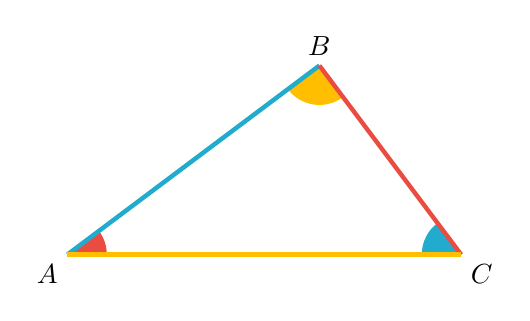
\begin{tikzpicture}
        \coordinate (A) at (0,0);
        \coordinate (B) at (3.2,2.4);
        \coordinate (C) at (5,0);
        \path[fill=red,ultra thick] (A) ++(0.5,0) arc (0:36:0.5) -- (A);
        \path[fill=yellow,ultra thick] (B) ++(-90+36:0.5) arc (-90+36:-180+36:0.5) -- (B);
        \path[fill=blue,ultra thick] (C) ++(-0.5,0) arc (180:90+36:0.5) -- (C);
        \node[below left ] at (A) {$A$};
        \node[above      ] at (B) {$B$};
        \node[below right] at (C) {$C$};
        \draw[blue,ultra thick]   (A) -- (B);
        \draw[red,ultra thick]    (B) -- (C);
        \draw[yellow,ultra thick] (C) -- (A);
    \end{tikzpicture}
    \end{figure}

    \begin{center}
        \textit{Some of the properties of the right angled triangle 
        \textrm{ABC}, expressed by the method generally employed.}
    \end{center}

    \begin{enumerate}
        \item The angle BAC, together with the angles BCA and ABC are 
            equal to two right angles, or twice the angle ABC. 
        \item The angle CAB added to the angle ACB will be equal to 
            the angle ABC. 
        \item The angle ABC is greater than either of the 
            angles BAC or BCA. 
        \item The angle BCA or the angle CAB is less than the 
            angle ABC. 
        \item If from the angle ABC, there be taken the angle BAC, 
            the remainder will be equal to the angle ACB. 
        \item The square of AC is equal to the sum of the squares 
            of AB and BC. 
    \end{enumerate}

    \begin{center}
        \textit{The same properties expressed by colouring 
        the different parts.}
    \end{center}

    \begin{enumerate}
        \item \[ \cab \plus \abc \plus \bca \equals 2\, \abc \equals \rightangles.\]
          That is, the red angle added to the yellow angle added to the blue angle, equal twice the yellow angle, equal two right angles. 
      \item \[\cab \plus \bca \equals \abc.\] 
          Or in words, the red angle added to the blue angle, equal the yellow angle. 
      \item \[\abc \greater \cab \text{ or } \greater \bca.\]
          The yellow angle is greater than either the red of blue angle. 
      \item \[\cab \text{ or } \bca \less\abc.\]
          Either the red or blue angle is less than the yellow angle.
      \item \[\abc \text{ minus } \bca \equals \cab.\]
          In other terms, the yellow angle made less by the blue angle equal the red angle. 
      \item \[\tikzhline[yellow]{1.2cm}^{2} \equals \tikzhline[blue]{1.2cm}^{2} \plus \tikzhline[red]{1.2cm}^{2}.\]
          That is, the square of the yellow line is equal to the sum of the squares of the blue and red lines. 
    \end{enumerate}

    In oral demonstrations we gain with colours this important advantage, the 
    eye and the ear can be addressed at the same moment, so that for teavhing 
    geometry, and other linear arts and sciences, in classes, the ststem is 
    the best ever proposed, this is apparent from the examples just 
    given. 

    Whence it is evident that a reference from the text to the diagram is more 
    rapid and sure, by giving the forms and colours of the parts, or by 
    naming the parts and their colours, than naming the parts and letters on 
    the diagram. Besides the superior simplicity, this system is likewise 
    conspicuous for concentration, and wholly excludes the injrious though 
    prevalent practice of allowing the student to commit the demonstration 
    to memory; until reason , and fact, and proof only make impressions on 
    the understanding. 

    Again, when lecturing on the principles or properties of figures, if we 
    mention the colour of the part or parts referred to, as in saying, the 
    red angle, the blue line, or lines, \&c.~the part or parts thus names 
    will be immediately seen by all in the class at the same instant; not so 
    if we say the angle ABC, the triangle PFQ, the figure EGKt, and so on; 
    for the letters must be traces one by one before the students arrange in 
    their minds the particular magnitude reeferred to, which often occasions 
    confusino and error, as well as lots of time. Also if the parts which are 
    given as equal, have the same colours in any diagram, the mind will not 
    wander from the object before it; that is, such an arrangement presents 
    an ocular demonstration of the parts to be proved equal, and the learner 
    retains the data throughout the whole of the reasoning. But whatever may 
    be the advantages of the present plan, if it be not substituted for, it 
    can always be made a powerful auxiliary to the other methods, for the 
    purpose of introduction, or of a more speedt reminiscence, or of more 
    permanent retention by the memory. 

    The experience of all who have formed systems to impress facts on the 
    understanding, agree in proving that coloured representations, as 
    pictures, cuts, diagrams, \&c.~are more easily fixed in the mind than 
    mere sentences unmarked by any peculiarity. Curious as it may appear, 
    poets seem to be aware of this fact more than mathematicians; many modern 
    poets allude to this visible system of communicating knowledge, one of 
    them has thus expressed himself: 
    \begin{quotation}
        Sounds which address the ear are lost and die\\
        In one short hour, but these which strike the eye,\\
        Live long upon the mind, the faithful sight\\
        Engraves the knowledge with a beam of light.
    \end{quotation}
    This perhaps may be reckoned the only improvement on which plain 
    geometry has recerived since the dats of Euclid, and if there were any 
    geometers of note before that time, Eclid's success has quite ecliped 
    their memory, and even occasioned all good things of that kindto be 
    assigned to him; like \AE sop among the writers of Fables. It may also be 
    worthy of remark, as tangible diagrams afford only the medium through 
    which geometry and other linear arts and scoences can be taught to the 
    blind, this visible system is no less adapted to the exigencies of the 
    deaf and dumb. 

    Care must be taken to show that colour has nothing to do with the lines, angles, or magnitudes except merely to name them. A mathematical line, which is length without breadth, cannot possess colour, yet the junction of two colours on the same plane gives a good idea of what is meant by a mathematical linel recorllect we are speaking familiarly, such a junction is to be understood and not the colour,l when we say the black line, the red line or line, \&c. 

    Colours and coloured diagrams may at first appear a climsy method to convery proper notions of the properties and parts of mathematical figures and magnitudes, however they will be found to afford a means more refined and extensive than any that has been hitherto proposed. 

    We shall here define a point, a line, and a sufrace, and demonstrate a proposition in order to show the truth of this assertion. 

    A spoint is that which has position, but not magnitude; or a point is position only, abstracted from the consideration of length, breadth, and thickness. Perhaps the following descriptiobn is better calculated to explain the nature of a mathematical point to those who have no acquired the idea, than the above specious definition. 

    Let three colours meet and cover a portion of the paper, where the meet is not blue, not is it yellow, not is it red, as it occupes no potion of the plane, for it it did, it would belong to the blue, the red or the yellow part; yet it exists, and has position without magnitude, so that with a little reflection , this junction of three colours on a plane, gives a good idea of a methamtical point. 
%   DIAGRAM OF A CIRCLE HERE
    A line is length withou breadth. With the assistance of colours, nearly inthe same manner as before, and idea of a line may be thus give:--

    Let two colours meet and cover a potion of the paper; where the meet is not red, nor is it blue; therefore it cannot have breadth, but only length: from which we can readily form an idea of what is meant by a mathematical line. For the purpose of illustration, one colour differing from the colour of the paper, or plane upon which it is drawn, would have been sufficient; hence in future, if we say the red line, the blue line, or line, \& c. it is the junctions with the plane upon which they are drawn are to be understood. 
%   DIAGRAM OF A PLANE HERE
    Surface is that which has length and breadth without thickness. 

    When we consider a solid body (PQ), we perceive at once that it has three dimensions, namely:-- length, breadth, and thickness; suppose one part of this solid (PS) to be red, and the other part (QR) yellow, and that the colours be distinct without commingling, the blue surface (RS) which separates these parts, or this is the same thing, that which divides the solid without loss of material, must be without thickness, and only possesses length and breadthl this plainly appears from reasoning, similar to that just employed in defining, or rather describing a point and a line. 
% Diagram of a cuboid here
    The proposition which we have selected to elucidate the manner in which the principles are applied, is the fifth proposition of the first Book. 
%COPY THE FIFTH PROPOSITION. 







    Our object in this place being to introduce the system rather than to teach any particular set of propositions, we have therefore selected the foregoing out of the regular course. For schools and other public places of instruction, dyed chalks will answer to describe diagrams, \&c. fo rprivate use coloured pencils will be found very convenient.
    We are happy to find that the Elements of Mathematics now forms a considerable part of ever found female education, therefore we call the attention of those interested or engaged in the education of ladies to this very attractive mode of communicating knowledge, and to the successing work for its future developement. 

    We shall for the present conclude by obsercing, as the sensed of sight and hearing can be so forcibly and instantaneously addressed alike with one thousand as with one, \textit{the million} might be taught geometry and other branches of mathematics with great ease, this would advance the purpose of education more than any thing that \textit{might} be names, for it would teach the people how to think, and not what to think; it is in this particular the great error of education originates.



 

    \newcounter{savepage}
    \setcounter{savepage}{\arabic{page}+1}
    \mainmatter
    \pagenumbering{roman}
    \setcounter{page}{\thesavepage}
    		{
		\cleardoublepage% Move to first page of new chapter
		\let\clearpage\relax% Don't allow page break
		{\hspace{48pt}\centering THE ELEMENTS OF EUCLID}%sorry
		
		\chapter{BOOK 1.}\label{book1}
		}
		\pagestyle{euclidbasic}
		{\centering\section{DEFINITIONS.}
		\label{section\thesection}
		}
		\begin{bizarrelist}
			\item A \textit{point} is that which has no parts.\label{def1}
			\item A \textit{line} is length without breadth.\label{def2}
			\item The extremities of a line are points. \label{def3}
			\item A straight or right line is that which lies evenly between its extermities.  \label{def4}
			\item A surface is that which has length and breadth only.   \label{def5}
			\item The extremities of a surface are lines.   \label{def6}
			\item A plane surface is that which lies evenly between its extremities.    \label{def7}
			\item A plane angle is the inclination of two lines to one another, in a plane, which meet together, but are not in the same direction.     \label{def8}
			\item A plane rectilinear angle is the inclination of two straight lines to one another, which meet together, but are not in the same straight line.     \label{def9}
			\item When one straight line standing on another straight linem makes the adjacent angles equal, each of these angles is called a right angle, and each of these lines is said to be perpendicular to the other.      \label{def10}
			\item An obtuse angle is an angle greater than a right angle.      \label{def11}
			\item An acute angle is an angle less than a right angle.       \label{def12}
			\item A term of boundary is the extremity of any thing.        \label{def13}
			\item A figure is a surface enclosed on all sides by a line or lines.         \label{def14}
			\item A circle is a plane figure, bounded by one continued line, called its circumference or periphery; and having a certain point within t, from which all straight lines drawn to its circumference are equal.          \label{def15}
			\item The point (from which the equal lines are drawn) is called the centre of the circle.           \label{def16}
			\item A diameter of a circle is a straight line drawn through the centre, terminating both ways in the circumference.            \label{def17}
			\item A semicircle is the figure contained by the diameter, and the part of the circle cut off by the diameter.            \label{def18}
			\item A segment of a circle is a figure contained by a straight line, and the part of the circumference which cuts it off.             \label{def19}
			\item A figure contained by straight lines only, is called a rectilinear figure.              \label{def20}
			\item A triangle is a rectilinear figure enclosed by three sides.               \label{def21}
			\item A quadrilateral figure is one which is bounded by four sides. The straight lines and connecting the vertices of the opposite angles of a quadrilateral figure, are called its diagonals.                \label{def22}
			\item A polygon is a rectilinear figure bounded by more than four sides.                 \label{def23}
			\item A traingle whose three sides are equal, is said to be equilateral.                  \label{def24}
			\item A triangle which has only two sides equal is called an isosceles triangle.                   \label{def25}
			\item A scalene triangle is one which has no two sides equal.                    \label{def26}
			\item A right angled triangle is that which has a right angle.                     \label{def27}
			\item An obtuse angled triangle is that which has an obtuse angle.                      \label{def28}
			\item An acute angled triangle is that which has three acute angles.                       \label{def29}
			\item Of four-sided figures, a square is that which has all its sides equal, and all its angles right angles.                        \label{def30}
			\item A rhombus is that which has all its sides equal, but its angles are not right angles.                         \label{def31}
			\item An oblong is that which has all its angles right angles, but has not all its sides equal.                          \label{def32}
			\item A rhomboid is that which has its opposite sides equal to one another, but all its sides are not equal, nor its angles right angles.                           \label{def33}
			\item All other quadrilateral figures are called trapeziums.                           \label{def34}
			\item Parallel straight lines are such as are in the same plane, and which being produced continually in both directions, would never meet.                            \label{def35}
		\end{bizarrelist}
		{\centering\section{POSTULATES.}
		\label{section\thesection}}
		\begin{bizarrelist}
			\item Let it be granted that a straight line may be drawn from any one point to any other point.\label{post1}
			\item Let it be granted that a finite straight line may be produced to any length in a straight line. \label{post2}
			\item Let it be granted that a circle may be described with any centre at any distance from that centre.  \label{post3}
		\end{bizarrelist}
		
		{\centering\section{AXIOMS.}
		\label{section\thesection}}
		\begin{bizarrelist}
			\item Magnitudes which are equal to the same are equal to each other. \label{ax1}
			\item If equals be added to equals the sums will be equal.  \label{ax2}
			\item If equals be taken away from equals the remainders will be equal.   \label{ax3}
			\item If equals be added to unequals the sums will be unequal.    \label{ax4}
			\item If equals be taken away from unequals the remainders will be unequal.     \label{ax5}
			\item The doubles of the same or equal magnitudes are equal.      \label{ax6}
			\item The halves of the same or equal magnitudes are equal.       \label{ax7}
			\item Magnitudes which coincide with one another, or exactly fill the same space, are equal.        \label{ax8}
			\item The whole is greater than its part.         \label{ax9}
			\item Two straight lines cannot include a space.          \label{ax10}
			\item All right angles are equal.           \label{ax11}
			\item If two straight lines 
				(
\begin{tikzpicture}[baseline=-0.5ex]
					\draw[blue,ultra thick] (0,-0.5ex) -- (1,-0.5ex);
					\draw[red,ultra thick] (0,0.5ex) -- (1,0.5ex);
				\end{tikzpicture}) 
				meet at a third straight line (\tikzhline{1cm}) so as to make the two interior angles (\tikzsector[yellow]{0}{-90}{1cm} and \tikzsector[blue]{0}{90}{1cm}) on the same side less than two right angles, these two straight lines will meet if they be produced on that side on which the angles are less than two right angles. \label{ax12}
		\end{bizarrelist}
		{\centering\section{ELUCIDATIONS.}
		\label{section\thesection}}
		The twelfth axiom may be expressed in any of the following ways: 
		\begin{enumerate}[itemsep=0pt]
			\item Two diverging straight lines cannot be both parallel to the same straight line. 
			\item If a straight line intersect one of the two parallel straight lines it must also intersect the other. 
			\item Only one straight line can be drawn through a given point, parallel to a given straight line. 
		\end{enumerate} 

		Geometry has for its principal object the exposition and explanation of the properties of \textit{figure}, and figure is defined to be the relation which subsists between the boundaries of space. Space or magnitude is of three kinds, \textit{linear}, \textit{superficial}, and \textit{solid}. 

		Angles might properly be considered as a fourth species of magnitude. Angular magnitude evidently consists of parts, and must therefore be admitted to be a species of quantity. The student must not suppose that the magnitude of an angle is affected by the length of the straight lines which include int, and of whose mutual divergence it is the measure. The \textit{vertex} of an angle is the point where the \textit{sides} or the \textit{legs} of the angle meet, as A. 

		An angle is often designated by a single letter when its legs are the only lines which meet together at its vertex. Thus the red and blue lines form the yellow angle, which in other systems would be called the angle A. But when more than two lines meet in the same point, it was necessary by former methods, in order to avoid confusion, to emplot three letters to designate an angle about that point, the letter which marked the vertex of the angle being always placed in the middle. thus the black and red lines meeting together at C, form the blue angle, and has been usually denominated the angle FCD or DCF. The lines FC and DC are the legs of the angle; the point C is its vertex. In like manner the black angle would be designated the angle DCB or BCD. The red and blue angles added together, or the angle HCF added to FCD, make the angle HCD; and so of other angles. 

When the legs of an angle are produced or prolonged beyond its vertex, the angles made by them on both ides of the vertex are said to be \textit{vertically opposite} to each other: Thus the red and tellow angles are said to be vertically opposite angles. 

\textit{Superposition} is the process by which one magnitude may be conceived to be placed upon another, so as exavtly to cover it, or so that every part os each shall exactly coincide. 

A line is said to be \textit{produced}, when it is extended, prolonged, or has its length increased, and the increase of length which it receives is called its \textit{produced part}, or its \textit{protrusion}. 

The entire length of the line or lines which enclose a figure, is called its perimeter. The first dix books of Euclid treat of plain figures only. A line drawn from the centre of a circle to its circumference, is called a \textit{radius}. The lines which include a figure are called its \textit{sides}. That side of a right angled triangle, which is opposite to the right angle, is called the \textit{hypotenuse}. An \textit{oblong} is defined in the second book, and called a \textit{recntagle}. All the lines which are considered in the first six books of the Elements are supposed to be in the same plane. 
The \textit{straight-edge} and \textit{compasses} are the only instruments, the use of which is permitted in Euclid, or plain Geometry. To declare this restriction is the object of the \textit{postulates}. 

The \textit{Axioms} of geometry are certain general propositions, the truth of which is taken to be self-evident and incapable of being established by demonstration. 

\textit{Propositions} are those results which are obtained in geometry by a process of reasoning. There are two species of propositions in geometry, \textit{problems} and \textit{theorems}. 

A \textit{Problem} is a proposition in which something is proposed to be done; as a line to be drawn under some given conditions, a circle to be described, some figure to be constructed, \&c. 

The \textit{Solution} of the problem consists in showing how the thing required may be done by the aid of the rule or straight-edge and compasses. 

The \textit{demonstration} consists in proving that the process indicated in the solution really attains the required end. 

A \textit{Theorem} is a proposition in which the truth of some principle is asserted. This principle must be deduced from the axioms and definitions, or other truths previouslu and independently established. To show this is the subject of demonstration. 

A \textit{Problem} is analogous to a postulate. 

A \textit{Theorem} resembles an axiom. 

A \textit{Postulate} is a problem, the solution of which is assumed. 

An \textit{Axiom} is a theorem, the truth os which is granted without demonstration. 

A \textit{Corollary} is an inference deduced immediately from a proposition. 

A \textit{Scholium} is a note or observation on a proposition not containing an inference of sufficient importance to entitle it to the name of \textit{corollary}. 

A \textit{Lemma} is a proposition merely introduced for the purpose of establishing some more important proposition. 

\begin{itemize}
\item[\therefore] expresses the word \textit{therefore}.
\item[\because] \manydots{10} \textit{because}.
\item[\equals] \manydots{10} \textit{equal}. This sign of equality may be read \textit{equal to}, or \textit{is equal to}, or \textit{are equal to}; but any discrepancy in regard to the introduction of the auxilliary verbs \textit{is, are, }\&c. cannot affect the geometrical rigour. 
\item[\notequals] means the same as if the words ``not equal'' were written.\item[\greater] signifies \textit{greater than}.
\item[\less] \manydots{4} \textit{less than}.
\item[\notgreater]\manydots{4} \textit{not greater than}.
\item[\notless]\manydots{4} \textit{not less than}. 
\item[\plus] is read \textit{plus} (\textit{more}), the sign of addition; and when placed between two magnitudes, signifies their sum. 
\item[\minus] is read \textit{minus} (\textit{less}), signifies subtraction; and when placed between two quantities denotes that the latter is to be taken from the former. 
\item[\cross] this sign expresses the product of two or more numbers when placed between them in arithmetic and algebra; but in geometry it is generally used to express a \textit{rectangle}, when placed between ``two straight lines which contain one of its right angles.'' A \textit{rectangle} may also be represented by placing a point between two of its counterminous sides. 
\item[\isto \as \isto] expresses an \textit{analogy} or \textit{proportion}; thus, if A, B, C and D, represent four magnitudes, and A has to B the same ratio that C has to D, the proposition is thus breifly written 
\begin{align*}
A \isto B &\as C \isto D,\\
A \isto B &\equals C \isto D,\\
\text{or } \frac{A}{B} &\equals \frac{C}{D}
\end{align*}
This equality or sameness of ratio is read 
\begin{center}
as A is to B, so C is to D; \\
or A is to B, as C is to D.
\end{center}
\item[\plel] signifies \textit{parallel} to. 
\item[\perpendicular] \manydots{4} \textit{perpendicular to}.
\item[\acuteangle] \manydots{1} \textit{angle}.
\item[\rightangle] \manydots{2} \textit{right angle}.
\item[\rightangles] \textit{two right angles}. 
\item[\trivertex or \vertex] briefly designates a \textit{point}.
\item[\greater,\equals or \less] signifies \textit{greater, equal, or less than}. 
\item[] The square described on a line is concisely written thus, ${\tikz[ultra thick,baseline=-0.5ex] \draw (0,0) -- (1,0);}^{2}$
\item[] In the same manner twice the square of, is expressed by $2 \cdot{\tikz[ultra thick,baseline=-0.5ex] \draw (0,0) -- (1,0);}^{2}$
\item[def.] signifies \textit{definition}.
\item[pos.] \manydots{4} \textit{postulate}.
\item[ax.] \manydots{4} \textit{axiom}.
\item[hyp.] \manydots{4} \textit{hypothesis}. It may be necessary here to remark, that the \textit{hypothesis} is the condition assumed or taken for gtanted. Thus, the hypothesis of the proposition given in the Introduction, is that the triangle is isosceles, or that its legs are equal. 
\item[const.] \manydots{4} \textit{construction}. The \textit{construction} is the change made in the original figure, by drawing lines, making angles, describing circle, \&c. om prder to adapt it to the argument of the demonstration or the solution of the problem. The conditions under which these changes are made, are as indisputable as those contained in the hypothesis. For instance, if we make an angle equal to a given angle, these two angles are equal by construction. 
\item[\qedsymbol]
\begin{tabular}[t]{ll}
\manydots{4}& \textit{Quod erat demonstratum}. \\ &Which was to be demonstrated. 
\end{tabular}
\end{itemize}
		\newpage
		{\centering\section[CORRIGENDA.]{\textit{Faults to be corrected before reading this Volume.}}
		\label{section\thesection}}
		\clearpage
        \pagenumbering{arabic}
        \setcounter{page}{1}
		{\centering\section{PROPOSITIONS.}
		\label{section\thesection}}

		\subsection{Proposition \the\numexpr \theprop + 1}
		
	\begin{prop}[problem]
%			\begin{cutout}{1}{0.5\textwidth}{0pt}{2}
			On a given finite straight line (\tikz[baseline=-0.5ex]\draw[ultra thick] (0,0) -- (1,0);) to describe an equlateral triangle.\\
			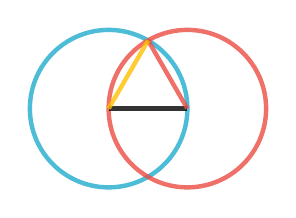
\begin{tikzpicture}[scale=1,opacity=0.8]
			\coordinate (A) at (0,0);
			\coordinate (B) at (1,0);
			\draw[name path=C1,blue,ultra thick] (A) circle (1cm);
			\draw[name path=C2,red,ultra thick] (B) circle (1cm);
			\path [name intersections={of=C1 and C2}];
			\coordinate (C) at (intersection-1);
			
			\draw[ultra thick] (A) -- (B); 
			\draw[ultra thick,red] (B) -- (C);
			\draw[ultra thick,yellow] (C) -- (A);
			\end{tikzpicture}
	%			text
%		\end{cutout}
	\end{prop}

	
	\begin{proof}
		Describe 
			
\begin{tikzpicture}[scale=0.5,opacity=0.8,baseline=-0.5ex]
			\coordinate (A) at (0,0);
			\coordinate (B) at (1,0);
			\draw[name path=C1,blue,ultra thick] (A) circle (1cm);
			\draw[ultra thick] (A) -- (B); 
			\end{tikzpicture}
		 and 
	 		
\begin{tikzpicture}[scale=0.5,opacity=0.8,baseline=-0.5ex]
	 		\coordinate (A) at (0,0);
	 		\coordinate (B) at (1,0);
	 		\draw[name path=C2,red,ultra thick] (B) circle (1cm);
	 		\draw[ultra thick] (A) -- (B); 
	 		\end{tikzpicture}
		 (\ref{post3}); draw \tikz[baseline=-0.5ex]\draw[yellow,ultra thick] (0,0) -- (1,0); and \tikz[baseline=-0.5ex]\draw[red,ultra thick] (0,0) -- (1,0); (\ref{post1}). then will 
	 	 		
\begin{tikzpicture}[baseline=-0.5ex,scale=0.5,opacity=0.8]
	 	 		\coordinate (A) at (0,0);
	 	 		\clip (-0.1,-0.1) rectangle (1.1,1.1);
	 	 		\coordinate (B) at (1,0);
	 	 		\path[name path=C1,blue,ultra thick] (A) circle (1cm);
	 	 		\path[name path=C2,red,ultra thick] (B) circle (1cm);
	 	 		\path [name intersections={of=C1 and C2}];
	 	 		\coordinate (C) at (intersection-1);
	 	 		\draw[ultra thick] (A) -- (B); 
	 	 		\draw[ultra thick,red] (B) -- (C);
	 	 		\draw[ultra thick,yellow] (C) -- (A);
	 	 		\end{tikzpicture}
		be equilateral. 
		\begin{align*}
			\text{For }  \tikz[baseline=-0.5ex]\draw[black,ultra thick] (0,0) -- (1,0); &= \tikz[baseline=-0.5ex]\draw[yellow,ultra thick] (0,0) -- (1,0);  (\text{ \ref{def15}})\\
			\text{and  }\tikz[baseline=-0.5ex]\draw[black,ultra thick] (0,0) -- (1,0); &= \tikz[baseline=-0.5ex]\draw[red,ultra thick] (0,0) -- (1,0); \text{ (\ref{def15})} \\
			\therefore \tikz[baseline=-0.5ex]\draw[yellow,ultra thick] (0,0) -- (1,0); &= \tikz[baseline=-0.5ex]\draw[red,ultra thick] (0,0) -- (1,0); \text{ (\ref{ax1})} 
		\end{align*}
	\end{proof}

		\clearpage
		\subsection{Proposition \the\numexpr \theprop + 1}
		
	\begin{prop}[Problem]
		\label{prop2}
		From a given point (
\begin{tikzpicture} [baseline=-0.5ex] \draw[red,ultra thick] (0,0) -- (0.6cm,0); \draw[blue,ultra thick] (0.6cm,0) -- (1cm,0);\end{tikzpicture}), 
			to draw a straight line equal to a given finite straight line (\tikzhline[black]{1cm}). % (\hline[black])	
	\end{prop}
	\begin{proof}
		Draw \tikzhline[densely dashed]{1cm} (\ref{post1}), describe 
		
\begin{tikzpicture}[scale=0.45,baseline=0.5ex]
			\draw[ultra thick,red] (0,0) -- (60:1) -- (1,0);
			\draw[ultra thick,densely dashed] (1,0) -- (0,0);
		\end{tikzpicture}
		(pr. 1.), produce \tikzhline[red]{0.7cm} (\ref{post2}), describe 
		
\begin{tikzpicture}[scale=0.4,baseline=-0.5ex]
			\draw[ultra thick] (0,0) -- (-1,0);
			\draw[blue,ultra thick] (0,0) circle (1cm);
		\end{tikzpicture}
		(\ref{post3}), and 
		
\begin{tikzpicture}[scale=0.4,baseline=-0.5ex]
			\draw[ultra thick,red] (0,0) -- (-60:0.4);
			\draw[ultra thick,yellow] (-60:0.4) -- (-60:1);
			\draw[ultra thick,red] (0,0) circle (1cm);
		\end{tikzpicture}

		(\ref{post3}); produce \tikzhline[red]{1cm} (\ref{post2}), then \tikzhline[blue]{1cm} is the line required. 
		For $
\begin{tikzpicture} [baseline=-0.5ex] \draw[yellow,ultra thick] (0,0) -- (0.6cm,0); \draw[red,ultra thick] (0.6cm,0) -- (1cm,0);\end{tikzpicture} = 
			
\begin{tikzpicture} [baseline=-0.5ex] \draw[red,ultra thick] (0,0) -- (0.4cm,0); \draw[blue,ultra thick] (0.4cm,0) -- (1cm,0);\end{tikzpicture}$
				(\ref{def15}), and $\tikzhline[red]{0.7cm} = \tikzhline[red]{0.7cm}$ (const.),
		$\therefore \tikzhline[yellow]{1cm} = \tikzhline[blue]{1cm}$ (\ref{ax3}), but (\ref{def15}) $\tikzhline[black]{1cm} = \tikzhline[yellow]{1cm} = \tikzhline[blue]{1cm}$;
		$\therefore \tikzhline[blue]{1cm}$ drawn from the given point 
		(
\begin{tikzpicture} [baseline=-0.5ex] \draw[red,ultra thick] (0,0) -- (0.4cm,0); \draw[blue,ultra thick] (0.4cm,0) -- (1cm,0);\end{tikzpicture}), 
			is equal the given line \tikzhline{1cm}.
		
	\end{proof}


		\clearpage
		\subsection{Proposition \the\numexpr \theprop + 1}
			\pagestyle{euclidprob}
    \begin{figure}[h]
        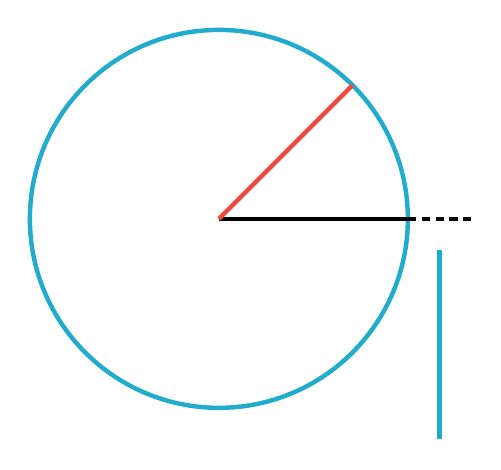
\begin{tikzpicture}[scale=0.8]
            \draw[ultra thick,blue] (0,0) circle (3cm);
            \draw[ultra thick,black] (0,0) -- (3,0);
            \draw[ultra thick,red] (0,0) -- (45:3cm);
            \draw[ultra thick,densely dashed] (3,0) -- (4,0);
            \draw[ultra thick,blue] (3.5,-0.5) -- (3.5,-3.5);
        \end{tikzpicture}
    \end{figure}

    \begin{prop}{\lettrine[lines=2]{F}rom}
		the greater (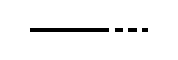
\begin{tikzpicture} 
			\draw[ultra thick] (0,0) -- (0.9cm,0);
			\draw[densely dashed,ultra thick] (0.9cm,0) -- (1.5cm,0);
		\end{tikzpicture}
			) of two straight lines , to cut a part off equal to the less (\tikzhline[blue]{0.9cm}).\par

	\end{prop}
	\begin{proof}
		Draw $\tikzhline[red]{1cm} = \tikzhline[blue]{1cm}$ (\refprop{2}); 
        describe 
        
\begin{tikzpicture}[scale=0.5]
            \draw[ultra thick,red] (0,0) -- (45:1.15cm);
            \draw[ultra thick,blue] (0,0) circle (1cm);
        \end{tikzpicture}
        (\refpost{3}), then $\tikzhline[blue]{0.9cm} \equals \tikzhline[black]{0.9cm}.$
        \begin{align*}
            \text{For } \tikzhline[red]{0.9cm} &\equals \tikzhline[black]{0.9cm} \text{ (\refdef{15})}, \\
            \text{and } \tikzhline[blue]{0.9cm} &\equals \tikzhline[red]{0.9cm} \text{ (const.)}; \\
            \therefore\, \tikzhline[blue]{0.9cm} &\equals \tikzhline[black]{0.9cm} \text{ (\refax{1})}. 
        \end{align*}
	\end{proof}

		\clearpage
		\subsection{Proposition \the\numexpr \theprop + 1}
			\pagestyle{euclidthm}
    \begin{figure}[h]
      \begin{subfigure}{0.35\textwidth}
        \begin{tikzpicture}[scale=0.8]
            \coordinate (C) at (0,0);
            \coordinate (B) at (4,1);
            \coordinate (A) at (3,4);
            \tikzsectorabc[fill=red]{(A)}{(B)}{(C)}{0.2}
            \tikzsectorabc[fill=blue]{(B)}{(C)}{(A)}{0.2}
            \tikzsectorabc[fill=yellow]{(C)}{(A)}{(B)}{0.2}
            \tikztriangle[blue][black][red]{(A)}{(B)}{(C)}
        \end{tikzpicture}
      \end{subfigure}
      \begin{subfigure}{0.35\textwidth}
        \begin{tikzpicture}[scale=0.8]
            \coordinate (C) at (0,0);
            \coordinate (B) at (4,1);
            \coordinate (A) at (3,4);
            \tikzsectorabc[fill=red]{(A)}{(B)}{(C)}{0.2}
            \tikzsectorabc[fill=blue]{(B)}{(C)}{(A)}{0.2}
            \tikzsectorabc[fill=yellow]{(C)}{(A)}{(B)}{0.2}
            \tikztriangle[blue][black][red]{(A)}{(B)}{(C)}
        \end{tikzpicture}
      \end{subfigure}
    \end{figure}

    \def\cab{
        \begin{tikzpicture}[scale=0.8]
            \coordinate (C) at (0,0);
            \coordinate (B) at (4,1);
            \coordinate (A) at (3,4);
            \tikzsectorabc[fill=yellow]{(C)}{(A)}{(B)}{0.2}
        \end{tikzpicture}
    }
    \def\abc{
        \begin{tikzpicture}[scale=0.8]
            \coordinate (C) at (0,0);
            \coordinate (B) at (4,1);
            \coordinate (A) at (3,4);
            \tikzsectorabc[fill=red]{(A)}{(B)}{(C)}{0.2}
        \end{tikzpicture}
    }
    \def\bca{
        \begin{tikzpicture}[scale=0.8]
            \coordinate (C) at (0,0);
            \coordinate (B) at (4,1);
            \coordinate (A) at (3,4);
            \tikzsectorabc[fill=blue]{(B)}{(C)}{(A)}{0.2}
        \end{tikzpicture}
    }
    \def\ab{\tikzhline[red]{0.5cm}}
    \def\bc{\tikzhline[blue]{0.5cm}}
    \def\ac{\tikzhline[black]{0.5cm}}
    \begin{prop}{\lettrine[lines=2]{I}f}
      two triangles have two sides of the one respectively equal to two 
      sides of the other, (\ac to \ac and \ab to \ab) and the angles (\cab 
      and \cab) contained by those equals sides also equal; then their 
      bases or their sides (\bc and \bc) are also equal: and the remaining 
      and their remaining angles opposite to equal sides are respectively 
      equal ($\bca \equals \bca$ and  $\abc \equals \abc$): and the triangles are equal in 
      every respect.
  \end{prop}
	\begin{proof}
    Let the two triangles be conceived, to be so placed, that the vertex 
    of the one of the equal angles, \cab or \cab ; shall fall upon that of 
    the other, and \ac to coincide with \ac, then will \ac coincide with \ac 
    is applied: consequently \bc will coincide with \bc, or two straight 
    lines will enclose a space, which is impossible (\refax{10}), therefore 
    $\bc = \bc$, 
	\end{proof}

		\clearpage
		\subsection{Proposition \the\numexpr \theprop + 1}
			\pagestyle{euclidthm}
    \newcommand{\coordspec}{
      \coordinate (A) at (0,5)    ;
      \coordinate (B) at (-3.5,-2);
      \coordinate (C) at (3.5,-2) ;
      \path (A) -- (B) node[coordinate,pos=0.6] (D) {D};
      \path (A) -- (C) node[coordinate,pos=0.6] (E) {E};
      \pgfresetboundingbox
    }
    \begin{figure}[h]
        \begin{tikzpicture}[scale=0.8]
            \coordspec
            \tikzsectorabc[fill=black]{(B)}{(A)}{(C)}{1cm}
            \tikzsectorabc[fill=blue]{(E)}{(D)}{(A)}{1cm}
            \tikzsectorabc[fill=blue]{(A)}{(E)}{(D)}{1cm}
            \tikzsectorabc[fill=yellow]{(C)}{(D)}{(E)}{1cm}
            \tikzsectorabc[fill=yellow]{(D)}{(E)}{(B)}{1cm}
            \tikzsectorabc[fill=red]{(E)}{(B)}{(A)}{1cm}
            \tikzsectorabc[fill=red]{(A)}{(C)}{(D)}{1cm}
            \tikztriangle[yellow][blue][red]{(A)}{(B)}{(E)}
            \tikztriangle[yellow][blue][red]{(A)}{(C)}{(D)}
            \tikztriangle[red][black][red]{(A)}{(D)}{(E)}
        \end{tikzpicture}
    \end{figure}
    \newcommand{\ADE}{
        \begin{tikzpicture}[scale=0.1]
            \coordspec
            \tikztriangle[red][black][red]{(A)}{(D)}{(E)}
            \pgfresetboundingbox
            \path (A) -- (D) -- (E) -- cycle;
        \end{tikzpicture}
    }
    \newcommand{\ABE}{
        \begin{tikzpicture}[scale=0.2,baseline=-0.5cm]
            \coordspec
            \tikzsectorabc[fill=black]{(B)}{(A)}{(C)}{0.3cm}
            \tikztriangle[yellow][blue][red]{(A)}{(B)}{(E)}
            \pgfresetboundingbox
            \path (A) -- (B) -- (E) -- cycle;
%            \draw[red,ultra thick] (E) -- (A) -- (D);
        \end{tikzpicture}
    }
    \newcommand{\ACD}{
        \begin{tikzpicture}[scale=0.2,baseline=-0.5cm]
            \coordspec
            \tikzsectorabc[fill=black]{(B)}{(A)}{(C)}{0.3cm}
            \tikztriangle[yellow][blue][red]{(A)}{(C)}{(D)}
            \pgfresetboundingbox
            \path (A) -- (C) -- (D) -- cycle;
%            \draw[red,ultra thick] (E) -- (A) -- (D);
        \end{tikzpicture}
    }
    \newcommand{\DEB}{
        \begin{tikzpicture}[scale=0.2]
            \coordspec
            \tikztriangle[black][blue][yellow]{(D)}{(E)}{(B)}
            \pgfresetboundingbox
            \path (D) -- (E) -- (B) -- cycle;
        \end{tikzpicture}
    }
    \newcommand{\EDC}{
        \begin{tikzpicture}[scale=0.2]
            \coordspec
            \tikztriangle[black][blue][yellow]{(E)}{(D)}{(C)}
            \pgfresetboundingbox
            \path (E) -- (D) -- (C) -- cycle;
        \end{tikzpicture}
    }
    \newcommand{\bac}{
      \begin{tikzpicture}
        \coordspec
        \tikzsectorabc[fill=black]{(B)}{(A)}{(C)}{0.5cm}
      \end{tikzpicture}
    }
    \newcommand{\abe}{
      \begin{tikzpicture}
        \coordspec
        \tikzsectorabc[fill=red]{(E)}{(B)}{(A)}{0.5cm}
      \end{tikzpicture}
    }
    \newcommand{\acd}{
      \begin{tikzpicture}
        \coordspec
        \tikzsectorabc[fill=red]{(A)}{(C)}{(D)}{0.5cm}
      \end{tikzpicture}
    }
    \newcommand{\adc}{
      \begin{tikzpicture}
        \coordspec
        \tikzsectorabc[fill=blue]{(E)}{(D)}{(A)}{0.5cm}
        \tikzsectorabc[fill=yellow]{(C)}{(D)}{(E)}{0.5cm}
      \end{tikzpicture}
    }
    \newcommand{\aeb}{
      \begin{tikzpicture}
        \coordspec
        \tikzsectorabc[fill=blue]{(A)}{(E)}{(D)}{0.5cm}
        \tikzsectorabc[fill=yellow]{(D)}{(E)}{(B)}{0.5cm}
      \end{tikzpicture}
    }
    \newcommand{\ade}{
      \begin{tikzpicture}
        \coordspec
        \tikzsectorabc[fill=blue]{(E)}{(D)}{(A)}{0.5cm}
      \end{tikzpicture}
    }
    \newcommand{\aed}{
      \begin{tikzpicture}
        \coordspec
        \tikzsectorabc[fill=blue]{(A)}{(E)}{(D)}{0.5cm}
      \end{tikzpicture}
    }
    \newcommand{\dec}{
      \begin{tikzpicture}
        \coordspec
        \tikzsectorabc[fill=white,draw=black]{(B)}{(E)}{(C)}{0.5cm}
        \draw (E) -- ($(E)!0.5cm!(C)$);
        \tikzsectorabc[fill=yellow]{(D)}{(E)}{(B)}{0.5cm}
      \end{tikzpicture}
    }
    \newcommand{\edc}{
      \begin{tikzpicture}
        \coordspec
        \tikzsectorabc[fill=yellow]{(C)}{(D)}{(E)}{0.5cm}
      \end{tikzpicture}
    }
    \newcommand{\deb}{
      \begin{tikzpicture}
        \coordspec
        \tikzsectorabc[fill=yellow]{(D)}{(E)}{(B)}{0.5cm}
      \end{tikzpicture}
    }
    \newcommand{\edb}{
      \begin{tikzpicture}
        \coordspec
        \tikzsectorabc[fill=white,draw=black]{(B)}{(D)}{(C)}{0.5cm}
        \draw (D) -- ($(D)!0.5cm!(B)$);
        \tikzsectorabc[fill=yellow]{(C)}{(D)}{(E)}{0.5cm}
      \end{tikzpicture}
    }
    \def\ab{
      \tikzhline[red]{0.5cm}\tikzhline[yellow]{0.5cm}
    }
    \def\ac{
      \tikzhline[red]{0.5cm}\tikzhline[yellow]{0.5cm}
    }
    \newcommand{\ad}{
      \tikzhline[red]{1cm}
    }
    \def\ae{
      \tikzhline[red]{1cm}
    }
    \newcommand{\db}{
      \tikzhline[yellow]{1cm}
    }
    \newcommand{\dc}{
      \tikzhline[blue]{1cm}
    }
    \newcommand{\eb}{
      \tikzhline[blue]{1cm}
    }
    \newcommand{\ec}{
      \tikzhline[yellow]{1cm}
    }

    

    \begin{prop}{\lettrine[lines=2]{I}n}
        any isosceles triangle \ADE if the equal sides be produced, the external angles at the base are equal, and the internal angles at the base are also equal. 
	\end{prop}
	\begin{proof}
        Produce \ad, and \ae, (\refpost{2}), take $\db \equals \ec$, (\refprop{3}); draw \dc and \eb. 

        Then in \ABE and \ACD we have, $\ab \equals \ac$ (const.), \bac common to both, and $\ad \equals \ae$ (hyp.) $\therefore \adc \equals \aeb$, $\dc \equals \eb$ and $\abe \equals \acd$ (\refprop{4}). Again in \DEB and \EDC we have $\db \equals \ec$, $\abe \equals \acd$ and $\dc \equals \eb$, \therefore\ $\edb \equals \dec$ and $\edc \equals \deb$  (\refprop{4}) but $\adc \equals \aeb$, $\therefore \ade \equals \aed$ (\refax{3}). 
	\end{proof}

		\clearpage


\end{document}
